\documentclass[letterpaper]{article}
\usepackage[submission]{aaai2027}
\usepackage[hyphens]{url}
\usepackage{graphicx}
\urlstyle{rm}
\def\UrlFont{\rm}
\usepackage{natbib}
\usepackage{caption}
\frenchspacing

\usepackage{amsmath,amssymb}
\usepackage{booktabs}
\usepackage{multirow}
\usepackage{algorithm}
\usepackage{algorithmic}

\newcommand{\cmark}{\textcolor{green!65!black}{\ensuremath{\checkmark}}}
\newcommand{\xmark}{\textcolor{red}{\ensuremath{\times}}}

\pdfinfo{
/TemplateVersion (2027.1)
}

\setcounter{secnumdepth}{0}

\title{ARMS: Routing by Model Capabilities for Evolving Vision-Language Model Pools}
\author{Anonymous Submission}
\affiliations{}

\begin{document}
\maketitle

\begin{abstract}
Vision-language models (VLMs) exhibit complementary, query-dependent strengths,
yet deployed systems often route every image-text request to one fixed model.
We study pre-invocation VLM routing. The router selects a candidate that is
likely to answer a query correctly before obtaining any candidate output. This problem
requires reasoning over both modalities and over heterogeneous model
capabilities, while candidate pools may change as new VLMs become available. We
introduce ARMS, a router that represents each candidate with a structured
description of its capabilities, fuses the image-text query through a gated
mixture of cross-attention experts, and matches the fused query representation
against each candidate description. We further propose incremental and
independent training strategies for adding previously unseen candidates without
retraining one router over the complete pool. Experiments on 56,107
answerable queries derived from four public multimodal benchmarks evaluate four
open-source and three commercial VLMs under in-distribution and
out-of-distribution shifts. ARMS improves answer-level Exact Match (EM) over every
individual candidate in both settings. In the separately evaluated, evolved
seven-model pool, independent training reaches 0.7958 in-distribution and 0.5428
out-of-distribution.
Ablations show that explicit candidate descriptions and gated multimodal fusion
are both necessary for accurate selection. These results establish routing with
explicit descriptions of model capabilities as an effective mechanism for
heterogeneous, evolving VLM pools.
\end{abstract}

\section{Introduction}

\begin{figure}[t]
  \centering
  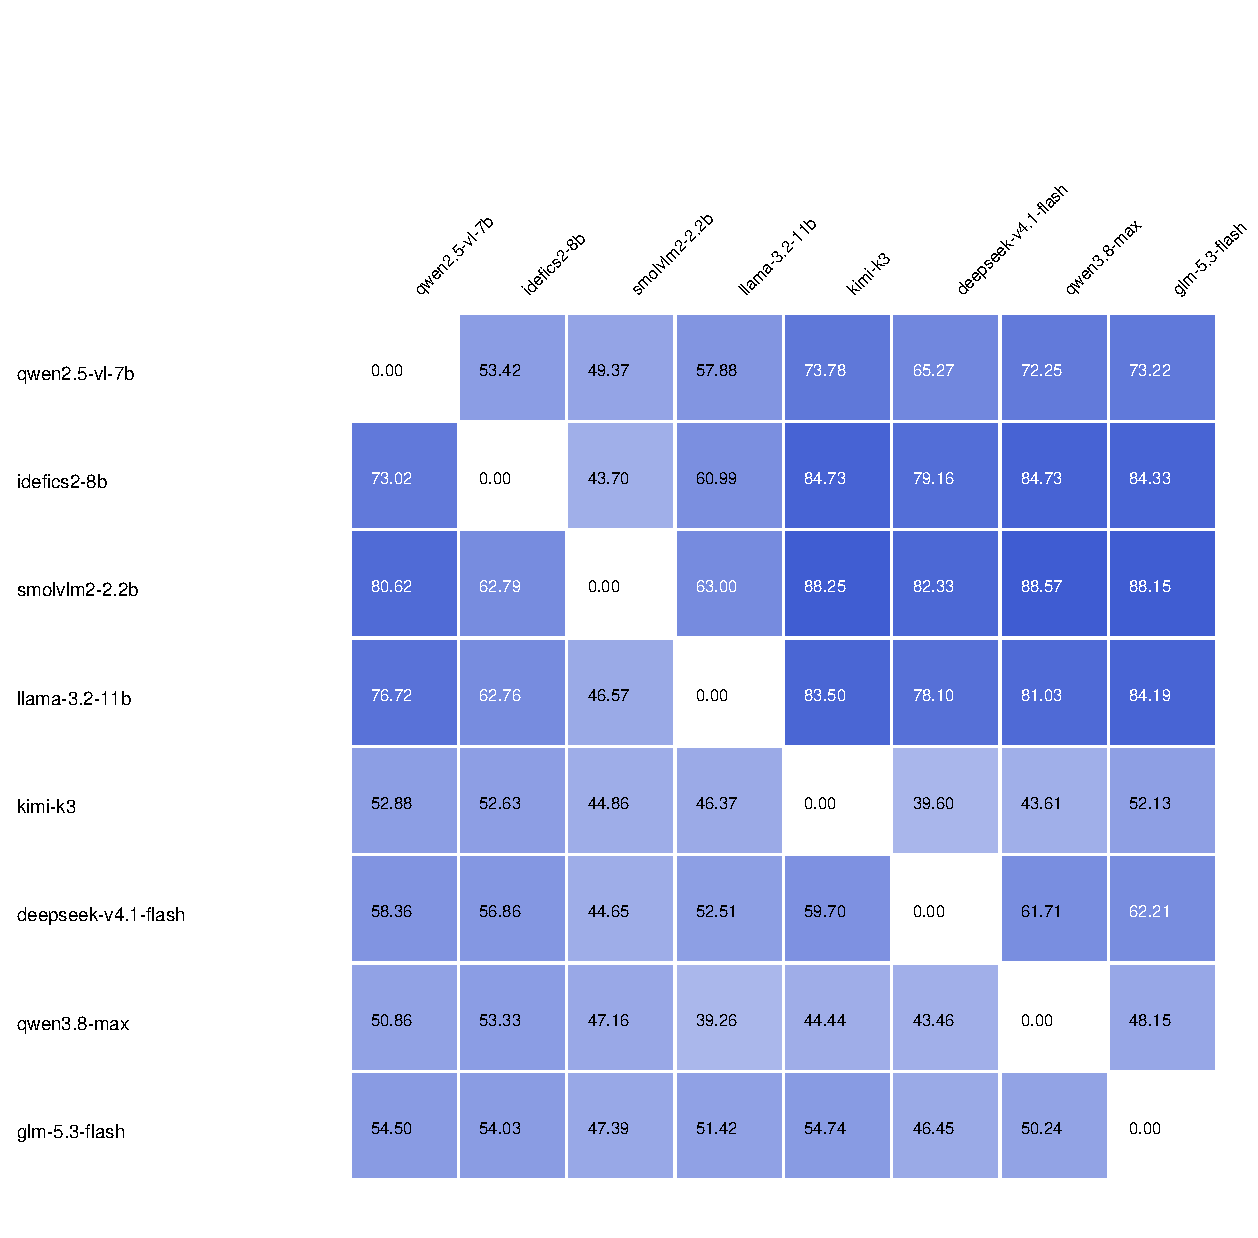
\includegraphics[width=0.98\columnwidth]{fig_outlined/heatmap.pdf}
  \caption{Percentage of VHELM queries missed by the row VLM but answered
  correctly by the column VLM. Off-diagonal values expose complementary
  capabilities that a router can exploit.}
  \label{fig:motivation}
\end{figure}

Vision-language models (VLMs) can answer the same image-text query with markedly
different accuracy. Empirical evaluations show that model scale and access mode
do not reliably identify the best candidate for a given query
\citep{VHELM,MARS}. Instead, differences in architecture, training data, and
modality backbones create complementary strengths in visual perception, OCR,
chart understanding, and multimodal reasoning. On VHELM \citep{VHELM}, for
example, Qwen2.5-VL-7B answers 52.88\% of the queries missed by kimi-k3, whereas
kimi-k3 answers 73.78\% of those missed by Qwen2.5-VL-7B (Figure~\ref{fig:motivation}).
This complementarity motivates query-level routing instead of using one VLM for
every request.

Existing language-model routers are not sufficient for this setting. First,
text-only routers cannot use the visual evidence that determines which VLM is
suitable. Second, a model identifier provides no explicit account of
the capabilities of each candidate. Third, routers trained for a fixed pool
encode decision boundaries tied to that pool and must be adapted when a new model
appears.
Together these issues define a distinct AI problem of multimodal,
query-level selection based on explicit model capabilities as the candidate pool
evolves.

We propose \textbf{ARMS}, a pre-invocation router for this problem. ARMS encodes
each candidate using a structured textual description of its capabilities and
encodes the query using text and image backbones. A learned gate weights cross-attention
experts that specialize the multimodal query representation. A matching head
then compares this representation with every candidate descriptor. Because the
score uses explicit model information rather than only a fixed output class,
the same formulation can accommodate new candidates. We operationalize an
evolving VLM pool by adding three
previously unseen VLMs to an original pool of four models. Incremental training
updates the original router using examples for the added VLMs, while independent
training learns a separate router and combines the two candidate subsets through
a confidence cascade.

Our contributions are threefold.
\begin{itemize}
  \item \textbf{Routing with explicit model capabilities.} We introduce a
  pre-invocation router that compares each image-text query with an explicit
  description of every candidate VLM's capabilities. Its shared scoring
  function is invariant to candidate order and retains the same output form as
  the pool grows.
  \item \textbf{Adapting as the VLM pool evolves.} ARMS uses a gate computed
  from the current query to combine cross-attention experts, then matches the
  fused query with cached embeddings of candidate descriptions. Incremental and
  independent training add previously unseen VLMs without retraining one router
  on all historical candidates.
  \item \textbf{Evaluation under distribution shifts.} We evaluate the original
  four-model pool and the evolved seven-model pool on 56,107 queries derived
  from four public multimodal benchmarks. Within each setting, ARMS outperforms
  every fixed candidate under both in-distribution (ID) and
  out-of-distribution (OOD) shifts; ablations isolate the effects of candidate
  descriptions, multimodal fusion, data balance, and cascade confidence.
\end{itemize}


\section{Related Work}

\paragraph{Pre- and post-invocation routing.}
Post-invocation methods use generated outputs as evidence. FrugalGPT evaluates
answers in a quality cascade \citep{FrugalGPT}, while LLM-Blender ranks and fuses
candidate responses \citep{LLM-Blender}. This evidence enables quality-aware
selection but requires at least one candidate invocation before the final
response and may increase latency. ARMS selects a candidate before observing any
output and therefore cannot use post-generation quality evidence; however, it
invokes no candidate VLM before selection. We claim no measured speedup because
we report neither wall-clock latency nor throughput.
Pre-invocation methods instead infer suitability from the request. FORC learns a
DistilBERT meta-scorer \citep{FORC}, TensorOpera Router uses a BERT selector
\citep{TO-Router}, and Hybrid LLM estimates query difficulty
\citep{Hybrid-LLM}. RouterDC jointly learns query and model embeddings using
sample--model and sample--sample contrastive objectives \citep{RouterDC}.
GraphRouter encodes task and model descriptions as node features in a
heterogeneous graph, enabling inductive routing to new models given auxiliary
interaction records \citep{GraphRouter}. Other approaches use nearest-neighbor
matching \citep{Routing} or reward-guided supervision \citep{ZOOTER}. ARMS
instead matches multimodal requests to candidate descriptions with a shared
pairwise function, without constructing an interaction graph or defining a
fixed class head.

\paragraph{Candidate representation and multimodal evidence.}
Prior routers encode candidates with learned embeddings, textual descriptions,
or graph-derived features. VHELM shows that relative VLM performance varies
across tasks, languages, and robustness conditions \citep{VHELM}. ARMS
summarizes documented architecture, scale, modality encoders, and reported
strengths in a compact textual descriptor. Whereas RouterDC uses learned
candidate embeddings, ARMS uses explicit descriptions; unlike GraphRouter, ARMS
does not construct a query--task--model graph. Cross-attention incorporates
visual evidence before the shared matcher scores each query--description pair.
Adding a descriptor does not alter the scoring head's dimensionality, although
observed query--candidate outcomes remain necessary for reliable adaptation.

\paragraph{Routing data and VLM evaluation.}
Table~\ref{tab:sources} contrasts routing resources by evidence and target.
RouterDC, MARS, and HELM release per-model outcomes for textual requests
\citep{RouterDC,MARS,HELM}, while VHELM supplies multimodal queries and VLM
outcomes for evaluation
\citep{VHELM}. The former do not expose visual routing evidence. The latter
samples at most roughly one thousand examples per task, which limits
in-distribution router training. We therefore derive query-candidate labels from
larger public multimodal benchmarks and reserve VHELM for transfer evaluation.
This protocol studies VLM routing without claiming a new standalone benchmark.

\begin{table}[t]
\centering
\footnotesize
\setlength{\tabcolsep}{1.7pt}
\begin{tabular}{lcccc}
\toprule
Dataset & Multimodal? & Model Outputs? & Target? & Queries\\
\midrule
FrugalGPT    & \xmark & \xmark & Selection  & 17,982\\
RouterDC     & \xmark & \cmark & Selection  & 8,225\\
MARS         & \xmark & \cmark & Selection  & 30,000\\
HELM         & \xmark & \cmark & Evaluation & 16,000\\
VHELM        & \cmark & \cmark & Evaluation & 21,000\\
ARMS (Ours)  & \cmark & \cmark & Selection  & 56,107\\
\bottomrule
\end{tabular}
\caption{Representative routing data sources compared along four dimensions.
``Model Outputs?'' denotes the availability of per-model outcomes, and
``Target?'' distinguishes selection resources from evaluation benchmarks.}
\label{tab:sources}
\end{table}

\section{Routing Corpus Construction}
\label{sec:corpus}

VLM routing requires supervision at the query-candidate level rather than only
an aggregate benchmark score. We construct this supervision from public
multimodal benchmarks in two stages. For the ID setting, we combine image-text
queries from ALM-Bench \citep{ALM-bench}, MMT-Bench \citep{MMT-Bench}, and
MME-RealWorld \citep{MME-RealWorld}. These sources cover multilingual
understanding, multi-task reasoning, and high-resolution real-world scenarios.
For OOD evaluation, we use VHELM \citep{VHELM}, whose constituent tasks and
sampling process differ from the ID sources. This split tests whether routing
patterns transfer beyond the benchmarks used to generate training pairs.

For each query, we invoke every available candidate and normalize its response
to the answer format required by the source benchmark. The label
$\bar y_{i,j}$ is one when candidate $V_j$ exactly matches the ground-truth
answer and zero otherwise. For each candidate pool, we retain query $i$ only if
at least one candidate is correct under the normalization rule.
\mbox{Oracle EM is 1.0 by construction.} This protocol does not evaluate detection or
abstention when every candidate fails. We split by query rather than by
query-candidate pair, ensuring that outcomes from the same query never appear
across training and test partitions.

We apply one answer normalization rule to every candidate. Multiple-choice prompts
request only the option letter; the parser extracts the first valid standalone
letter and compares it case-insensitively with the reference. For free-form
answers, normalization removes leading and trailing whitespace, lowercases the
text, and collapses consecutive whitespace before strict equality. It does not
use semantic or substring matching. These fixed rules prevent processing
tailored to individual models from changing the routing labels.

The four-model pool yields four outcomes per retained query. To study pool
evolution, we query three commercial VLMs on a disjoint ID subset and form
training pairs for the added candidates. OOD sets are never used for optimization
or threshold selection. The experiments on the evolved pool therefore change
both the candidate set and the query set. We compare ARMS with baselines that
always select one candidate within each setting rather than attributing score
differences across settings to pool growth. We call this resource a routing corpus because
its queries and annotations come from public benchmarks. The contribution is the
routing method and evaluation protocol.

Figure~\ref{fig:sample} shows one labeled pair containing an image, a question,
and a shared output-format instruction. Comparing the candidate response with
the green reference yields label zero. Storing candidate outcomes separately
lets one image-text query supervise multiple suitability decisions.

\begin{figure}[t]
  \centering
  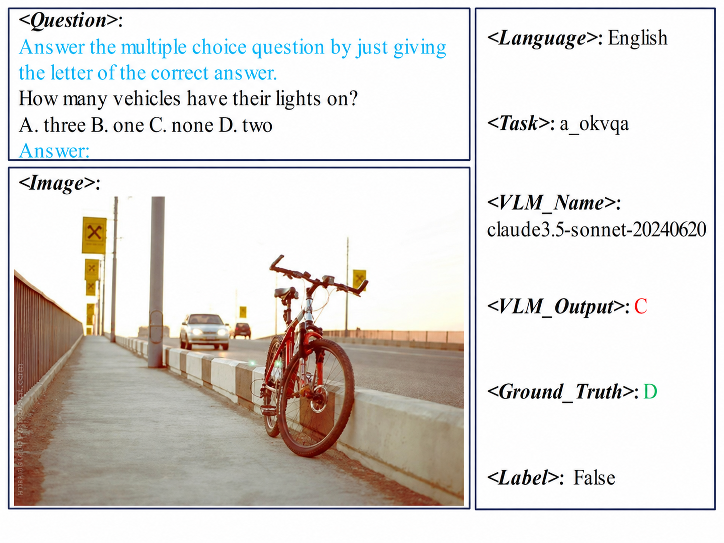
\includegraphics[width=0.88\columnwidth]{fig_outlined/sample.pdf}
  \caption{One query-candidate pair used for routing supervision. Blue text is
  the standardized output instruction, green is the reference answer, and red
  is the candidate response.}
  \label{fig:sample}
\end{figure}

\section{VLM Routing with Explicit Capability Descriptions}
\label{sec:method}

\subsection{Problem Formulation}

{\hyphenpenalty=10000
Let $x_i=(Q_i,G_i)$ be a query containing question $Q_i$ and image $G_i$, and
let $\mathcal{S}=\{V_1,\ldots,V_K\}$ be the candidate VLMs. Candidate $V_j$ is
paired with descriptor $M_j$, a short text containing its name, parameter count,
architecture, language and vision backbones, and documented task strengths.
Before invoking a candidate, the router predicts
$c_{i,j}=p_{\Phi}(\bar y_{i,j}=1\mid Q_i,G_i,M_j)$, where $\bar y_{i,j}=1$ iff
$V_j$ answers query $i$ correctly. It selects
$V^*=\arg\max_{V_j\in\mathcal{S}}c_{i,j}$ and minimizes binary cross-entropy
over all observed query-candidate pairs.\par}
\small
\begin{equation}
\mathcal{L}(\Phi)=-\sum_i\sum_{j=1}^{K}\!\left[
\bar y_{i,j}\log c_{i,j}+(1-\bar y_{i,j})\log(1-c_{i,j})\right].
\label{eq:objective}
\end{equation}
\normalsize
Routing quality is measured by the correctness of the selected VLM's answer.
Classification metrics diagnose the pairwise suitability predictor.

\subsection{Encoding Queries and Candidate Capabilities}

As illustrated in Figure~\ref{fig:architecture}, a shared BERT-based encoder maps
$Q_i$ and $M_j$ to $q_i\in\mathbb{R}^{d_q}$ and
$m_j\in\mathbb{R}^{d_m}$. A CLIP image encoder maps $G_i$ to visual tokens
$g_i=[g_{i,1},\ldots,g_{i,L}]^\top\in\mathbb{R}^{L\times d_g}$, with pooled
vector $\bar g_i=L^{-1}\sum_{\ell}g_{i,\ell}$. Keeping visual tokens rather
than only a global embedding allows the query representation to attend to
image regions relevant to the question.

The descriptor schema is deliberately compact (Table~\ref{tab:descriptor}).
Identity and scale distinguish candidate versions. Architecture and backbone
fields expose how the model processes the two modalities. The capability summary
captures documented strengths in natural language. All fields form one text
sequence, enabling a new descriptor to be scored without changing the
dimensionality of the matching head.

The same field order is used for open-source and commercial VLMs. A descriptor
contains no response to the current query and is encoded once before routing,
so the decision remains pre-invocation. The text supplies model side
information; it does not replace behavioral supervision. Query-candidate
outcomes are still needed to learn how documented attributes relate to success
on actual visual questions, especially after a previously unseen VLM is added.

\begin{table}[t]
\centering
\begin{tabular}{ll}
\toprule
Descriptor field & Information represented\\
\midrule
Identity & Model name and version\\
Scale & Parameter count\\
Architecture & VLM architecture family\\
Vision backbone & Image encoder family\\
Language backbone & Language model family\\
Capability summary & Documented task strengths\\
\bottomrule
\end{tabular}
\caption{Fixed schema used to describe each candidate VLM.}
\label{tab:descriptor}
\end{table}

\begin{figure}[t]
  \centering
  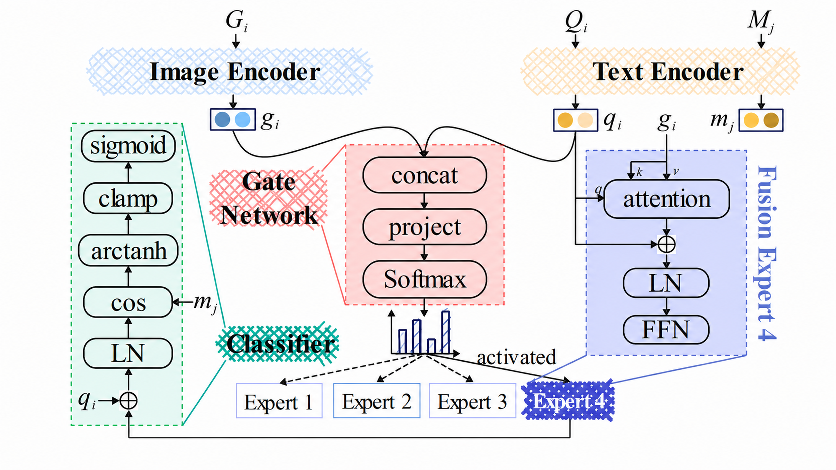
\includegraphics[width=\columnwidth]{fig_outlined/arms.pdf}
  \caption{ARMS encodes the multimodal query and each candidate description,
  fuses query features with gated cross-attention experts, and predicts whether
  each candidate can answer correctly.}
  \label{fig:architecture}
\end{figure}

\subsection{Gated Cross-Attention Experts}

A gate computed from the current query softly weights $N$ fusion experts.
\begin{equation}
p_i=\operatorname{softmax}\!\left(W_{\rm gate}[q_i;\bar g_i]+b_{\rm gate}\right).
\label{eq:gate}
\end{equation}
Expert $n$ projects both modalities to dimension $d_a$ and uses the question
to attend to visual tokens.
\begin{align}
u_i^{(n)}&=W_Q^{(n)}q_i, \quad K_i^{(n)}=g_iW_K^{(n)},
\quad H_i^{(n)}=g_iW_V^{(n)},\nonumber\\
a_i^{(n)}&=\operatorname{softmax}\!\left(
\frac{(u_i^{(n)})^\top(K_i^{(n)})^\top}{\sqrt{d_a}}\right)H_i^{(n)},\nonumber\\
e_i^{(n)}&=\operatorname{FFN}_n\!\left(\operatorname{LN}_n
([q_i;a_i^{(n)}])\right),\qquad
e_i=\sum_{n=1}^{N}p_i^{(n)}e_i^{(n)}.
\label{eq:experts}
\end{align}
Soft weighting preserves gradient flow to every expert while allowing
specialization by query type.

\subsection{Matching Queries to Candidate Descriptions}

The router matches each fused query to an embedding of the candidate description
by cosine similarity.
\small
\begin{equation}
h_i=W_h\operatorname{LN}([q_i;e_i])+b_h,\qquad
s_{i,j}=\frac{h_i^\top m_j}{\lVert h_i\rVert_2\lVert m_j\rVert_2}.
\end{equation}
\normalsize
For finite logits, we clip the cosine and bound its inverse-hyperbolic tangent.
\small
\begin{align}
\tilde s_{i,j}&=\operatorname{clip}(s_{i,j},-1+\epsilon,1-\epsilon),\nonumber\\
z_{i,j}&=\operatorname{clip}(\operatorname{arctanh}(\tilde s_{i,j}),
\ell_{\min},\ell_{\max}),\quad c_{i,j}=\sigma(z_{i,j}).
\label{eq:score}
\end{align}
\normalsize
The resulting score is the probability used in
Equation~\ref{eq:objective}.

Candidate-description embeddings $m_j$ are query-independent and cached. ARMS
encodes each image-text query once, evaluates $N$ experts, and compares the
resulting representation with every cached descriptor. It invokes no candidate
VLM before selection. Only the final matching term grows linearly with
$|\mathcal{S}|$; adding a descriptor leaves the scoring-head dimensionality
unchanged.

\subsection{Properties of Shared Candidate Scoring}

ARMS uses one shared scoring function $f_{\Phi}(x_i,M_j)$ for every candidate,
rather than a $K$-way classification head whose coordinates are tied to a fixed
pool. Consequently, permuting candidate order leaves every pairwise score and
the selected argmax unchanged. Increasing $K$ also leaves the learned output
shape unchanged. A new descriptor can be encoded and compared in the same
space. This property enables extensibility, but it does not imply reliable
zero-shot routing to an arbitrary new VLM. The new descriptor and outcome data
may lie outside the learned distribution, which is why the two strategies below
adapt the scoring function or add a separately calibrated scorer.

Let $C_{\rm enc}$ denote the computational cost of the text and image encoders,
$C_{\rm att}$ the computational cost of one fusion expert, and $d_m$ the
matching dimension.
With cached embeddings of candidate descriptions, per-query complexity is
\begin{equation}
O(C_{\rm enc}+N C_{\rm att}+K d_m).
\end{equation}
The expensive multimodal query encoding is shared across candidates. Only the
final matching term grows with the pool. The gate also depends on the query,
not the ordering of candidates, so all candidates are compared against the same fused
evidence. These invariances distinguish matching with explicit candidate
descriptions from a router with a fixed set of classes and explain why the
original scoring semantics can be preserved as the pool evolves.

\subsection{Routing as the VLM Pool Evolves}

Let $\mathcal{S}_{\rm new}$ contain VLMs unavailable during initial training.
\emph{Incremental training} initializes from router $\Phi$ and continues
optimization on training pairs for the added candidates, denoted by
$D_{\rm new}$, producing parameters
$\Phi+\Delta\Phi$ by minimizing
\begin{equation}
\mathcal{L}_{\rm inc}(\Delta\Phi)=
-\sum_{(x_i,V_j)\in D_{\rm new}}
\log p_{\Phi+\Delta\Phi}(\bar y_{i,j}\mid x_i,M_j).
\label{eq:incremental}
\end{equation}
This update is inexpensive and retains the original representation, but it can
be sensitive to imbalance between data for the original and added VLMs.

\emph{Independent training} learns router $\Theta$ only on $D_{\rm new}$. At
inference, $\Phi$ first scores the original pool. Let
$c_{\rm old}=\max_{V_j\in\mathcal{S}}c_{i,j}^{\Phi}$ and let $V_{\rm old}$ be
its maximizer. If $c_{\rm old}>\theta$, ARMS selects $V_{\rm old}$. Otherwise,
$\Theta$ scores $\mathcal{S}_{\rm new}$ and ARMS selects the candidate with the
largest confidence across the two subsets. The threshold therefore trades early
acceptance from the established pool against consultation of the new router.
This cascade avoids parameter interference between heterogeneous candidate
groups and requires no joint pass over all historical data.

Algorithm~\ref{alg:extension} summarizes the independent inference rule. The
highest-scoring VLM from the original pool remains a candidate, while its score
determines early acceptance. If early acceptance does not occur, the router for
the added VLMs is consulted and the two maxima are compared on the same
confidence scale.

\begin{algorithm}[t]
\caption{Independent Training as the VLM Pool Evolves}
\label{alg:extension}
\begin{algorithmic}[1]
\REQUIRE Query $x$, routers $\Phi,\Theta$, pools $\mathcal{S},\mathcal{S}_{\rm new}$,
threshold $\theta$
\ENSURE Selected candidate $V^*$
\STATE $(V_o,c_o)\leftarrow\arg\max_{V\in\mathcal{S}}c^{\Phi}(x,V)$
\IF{$c_o>\theta$}
  \STATE $V^*\leftarrow V_o$
\ELSE
  \STATE $(V_n,c_n)\leftarrow\arg\max_{V\in\mathcal{S}_{\rm new}}c^{\Theta}(x,V)$
  \STATE $V^*\leftarrow V_o$ if $c_o\geq c_n$, otherwise $V_n$
\ENDIF
\end{algorithmic}
\end{algorithm}

\begin{figure*}[t]
  \centering
  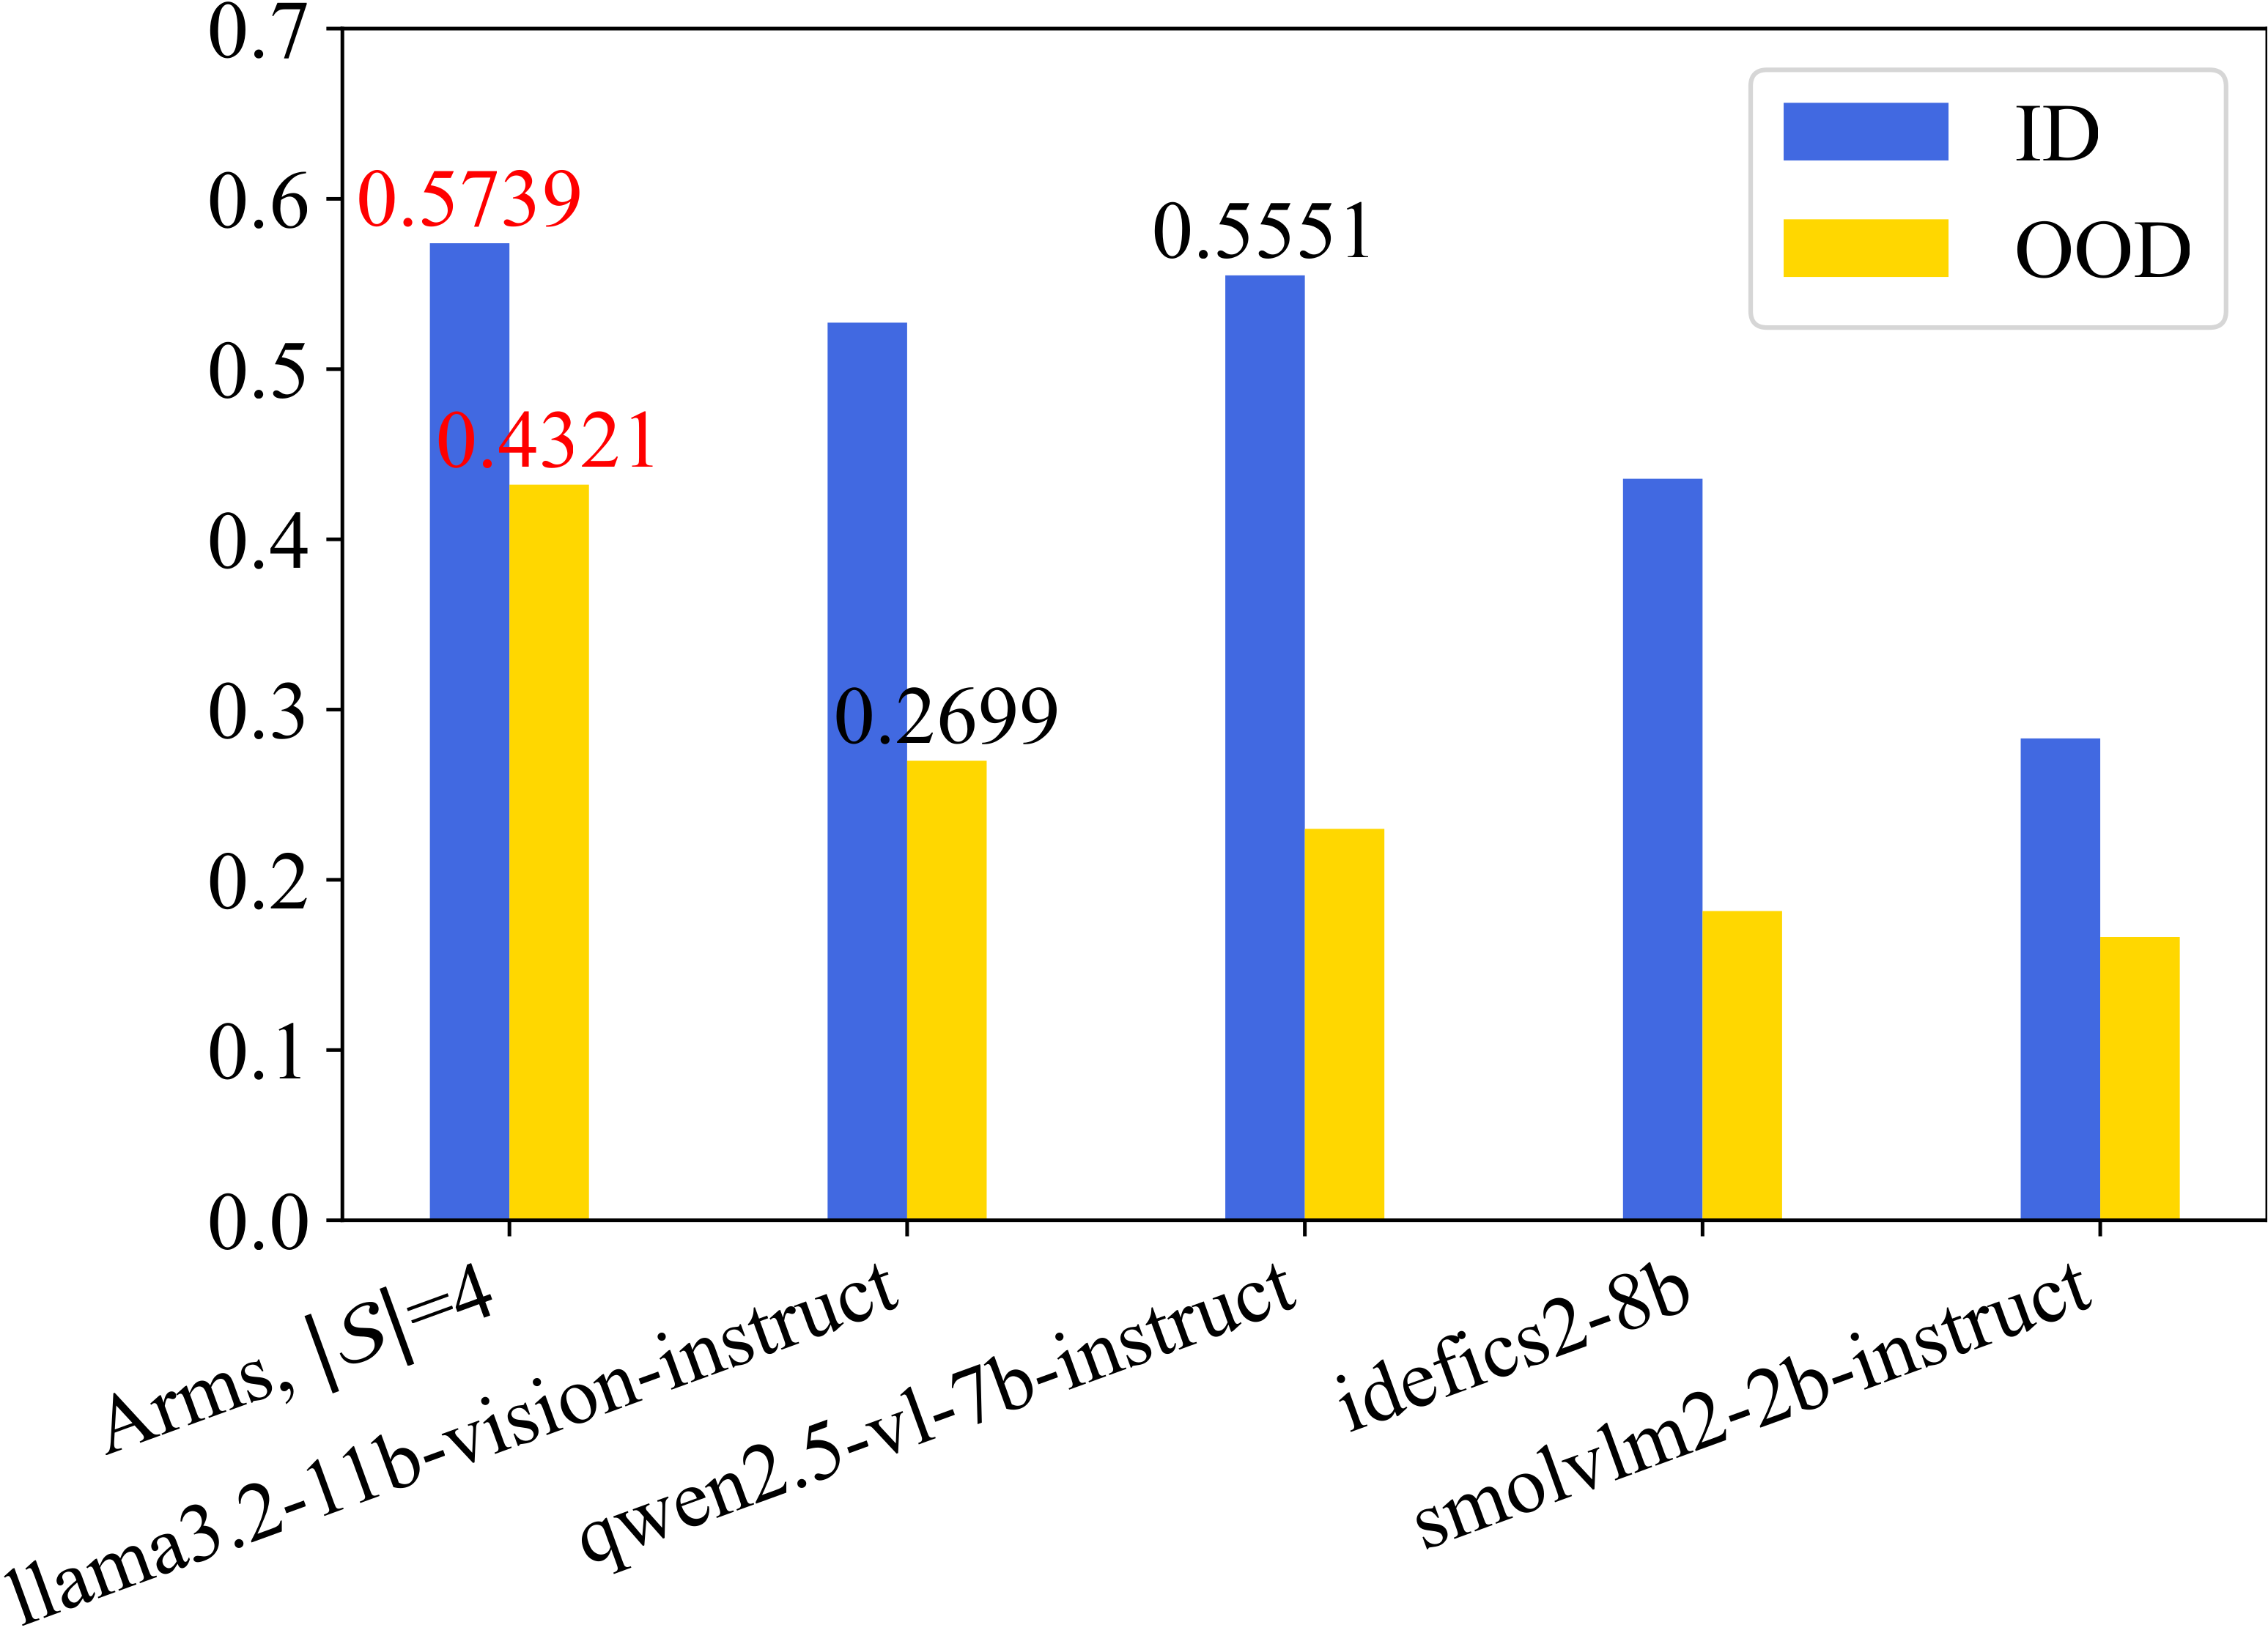
\includegraphics[width=0.39\textwidth]{fig_outlined/4vlm-em.png}\hfill
  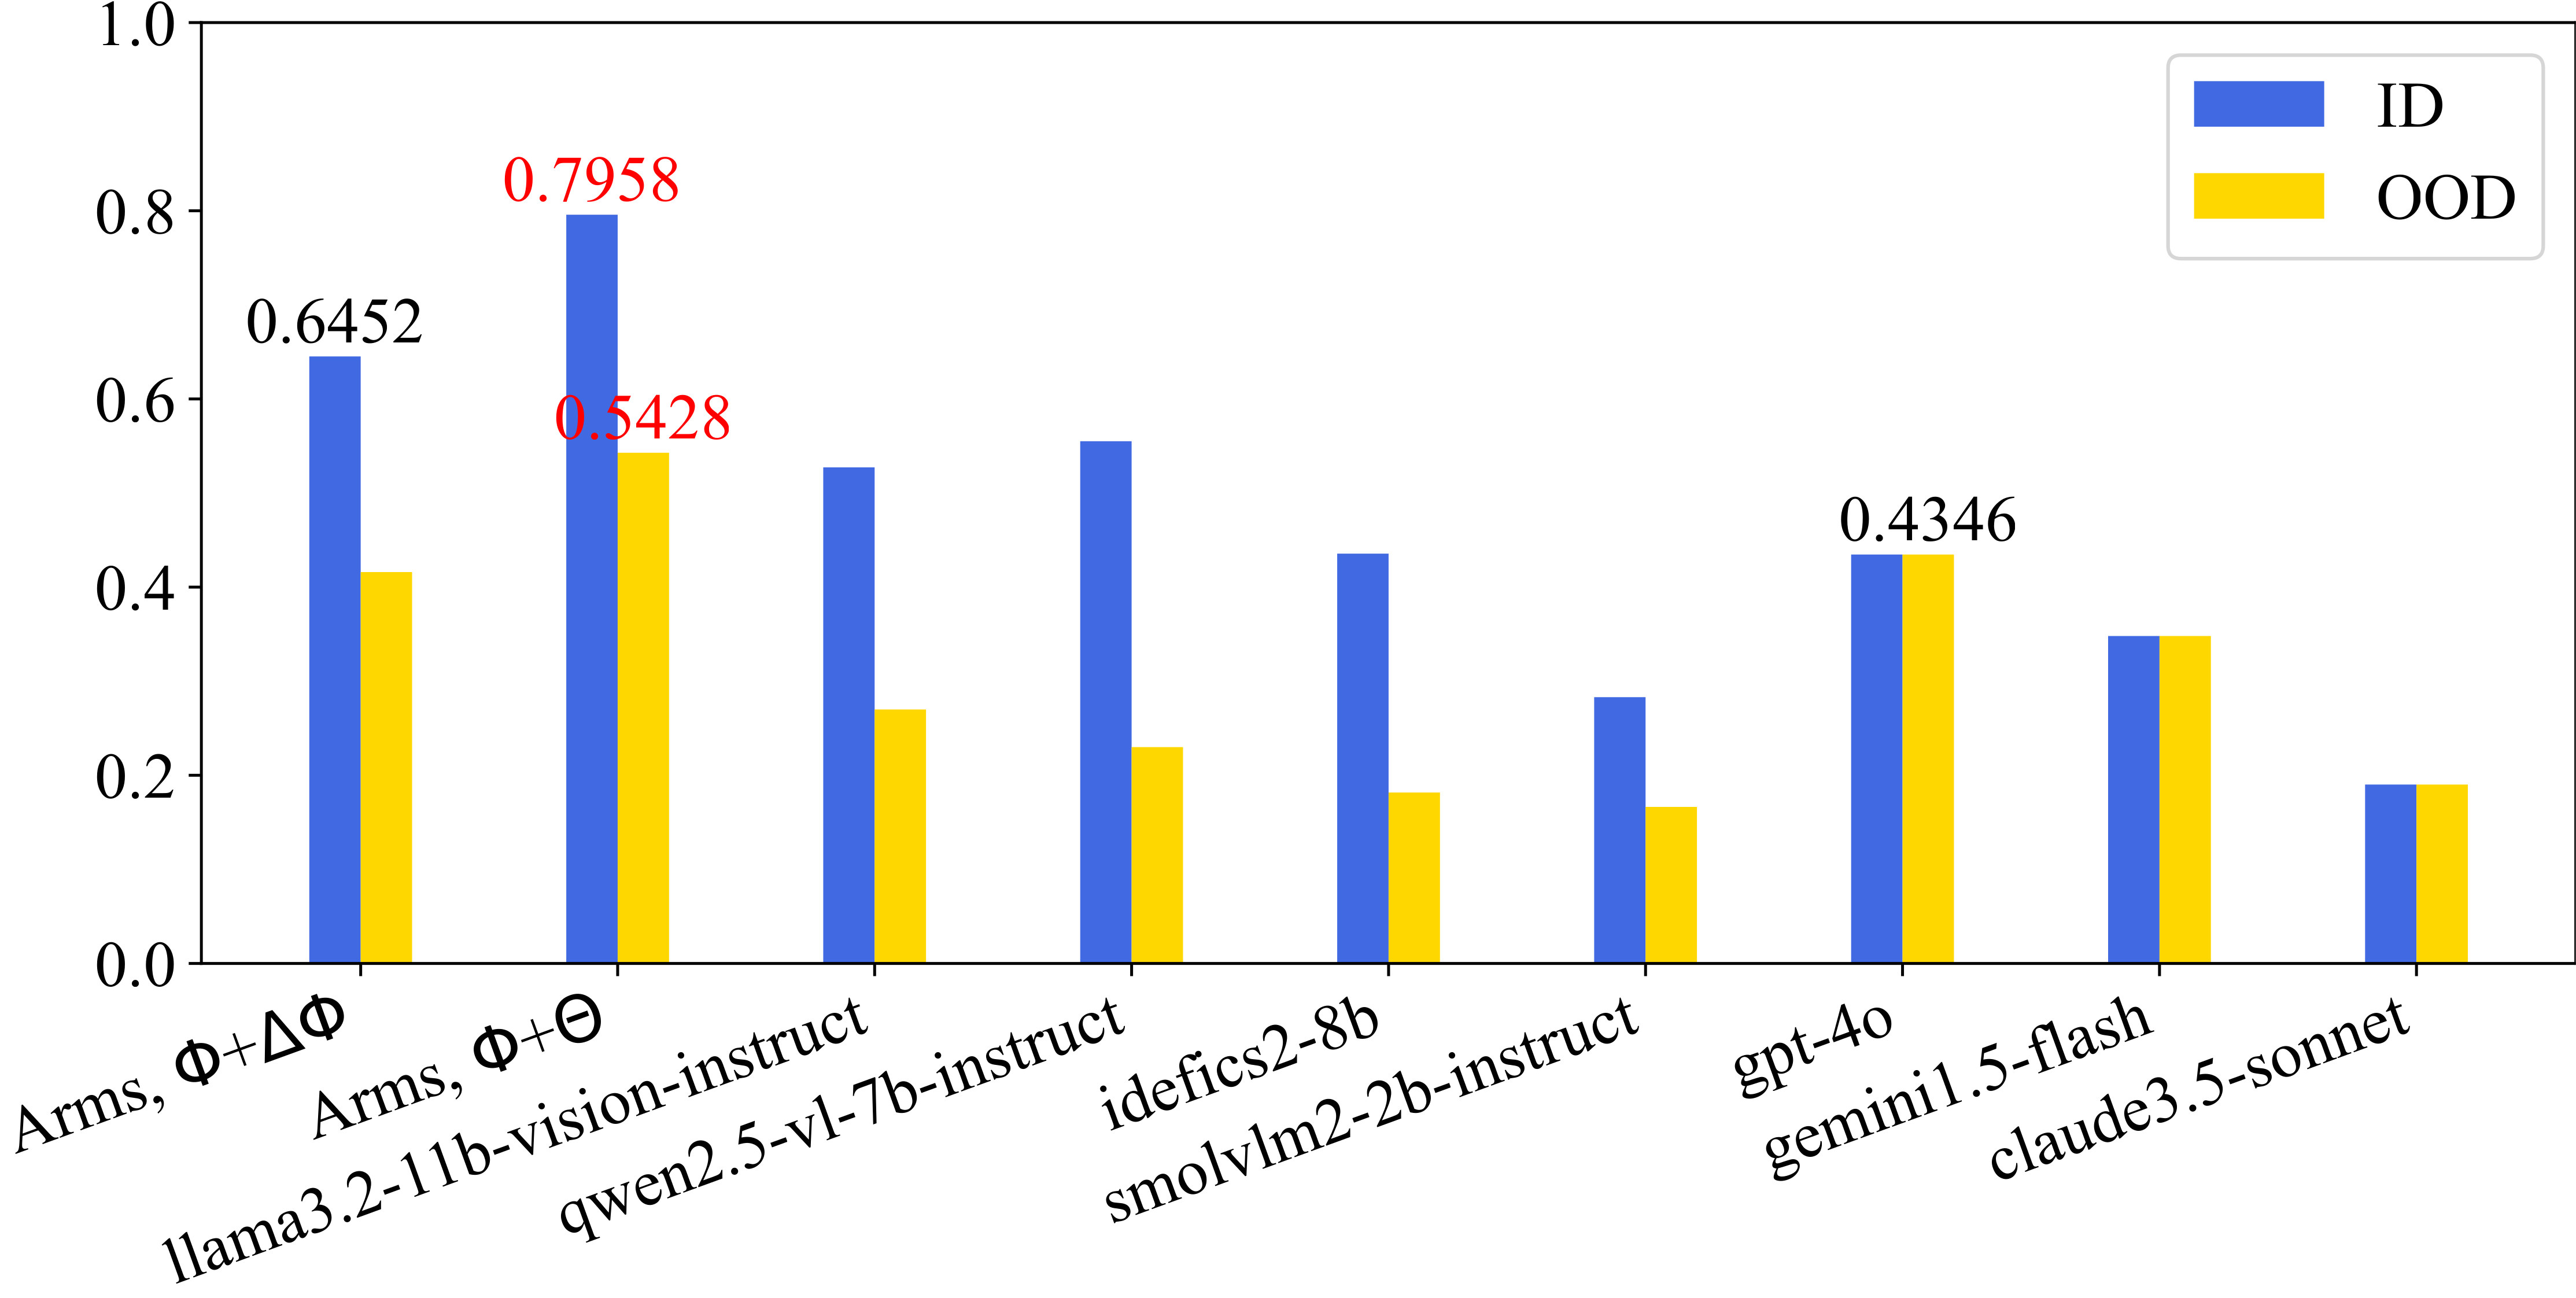
\includegraphics[width=0.57\textwidth]{fig_outlined/7vlm-em.png}
  \caption{Answer-level EM for (left) the original four-model pool and (right)
  the separately evaluated, evolved seven-model pool. $\Phi+\Delta\Phi$ denotes
  incremental training and $\Phi+\Theta$ denotes independent training. Within
  each setting, ARMS exceeds every fixed candidate in both ID and OOD
  evaluations. Oracle EM is 1.0 by construction.}
  \label{fig:main}
\end{figure*}

\begin{figure*}[t]
  \centering
  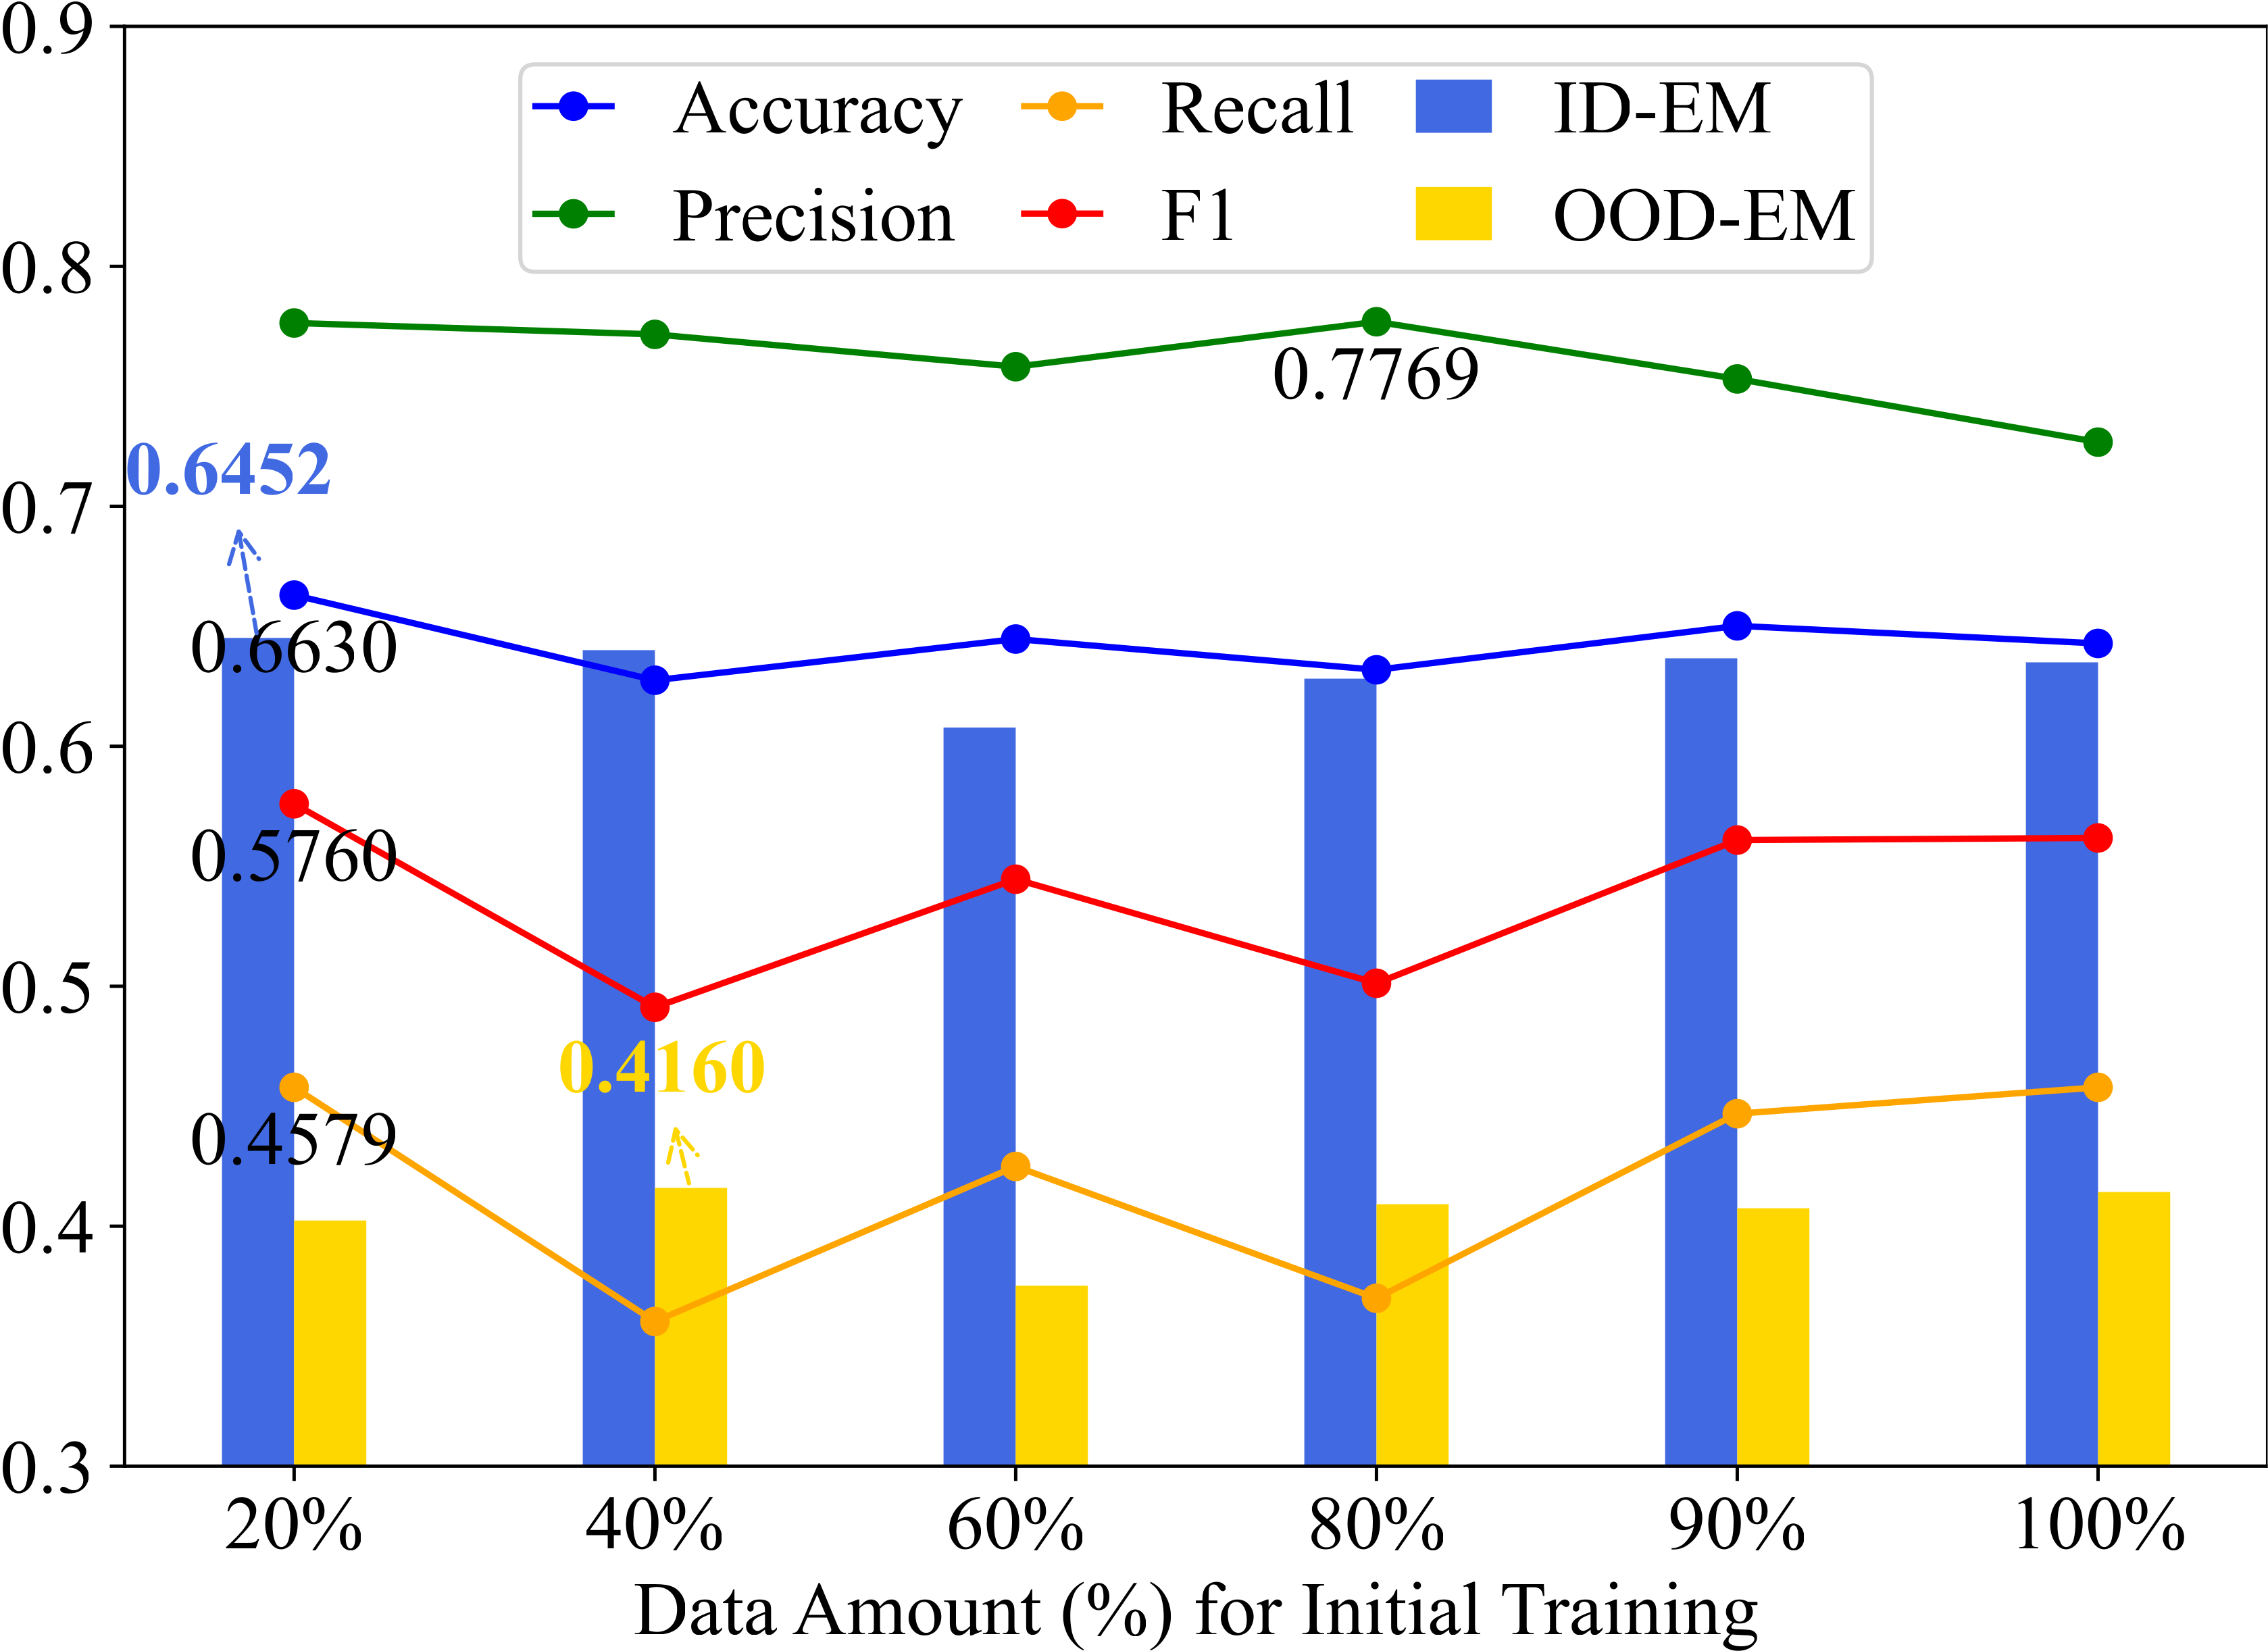
\includegraphics[width=0.465\textwidth]{fig_outlined/incremental.png}\hfill
  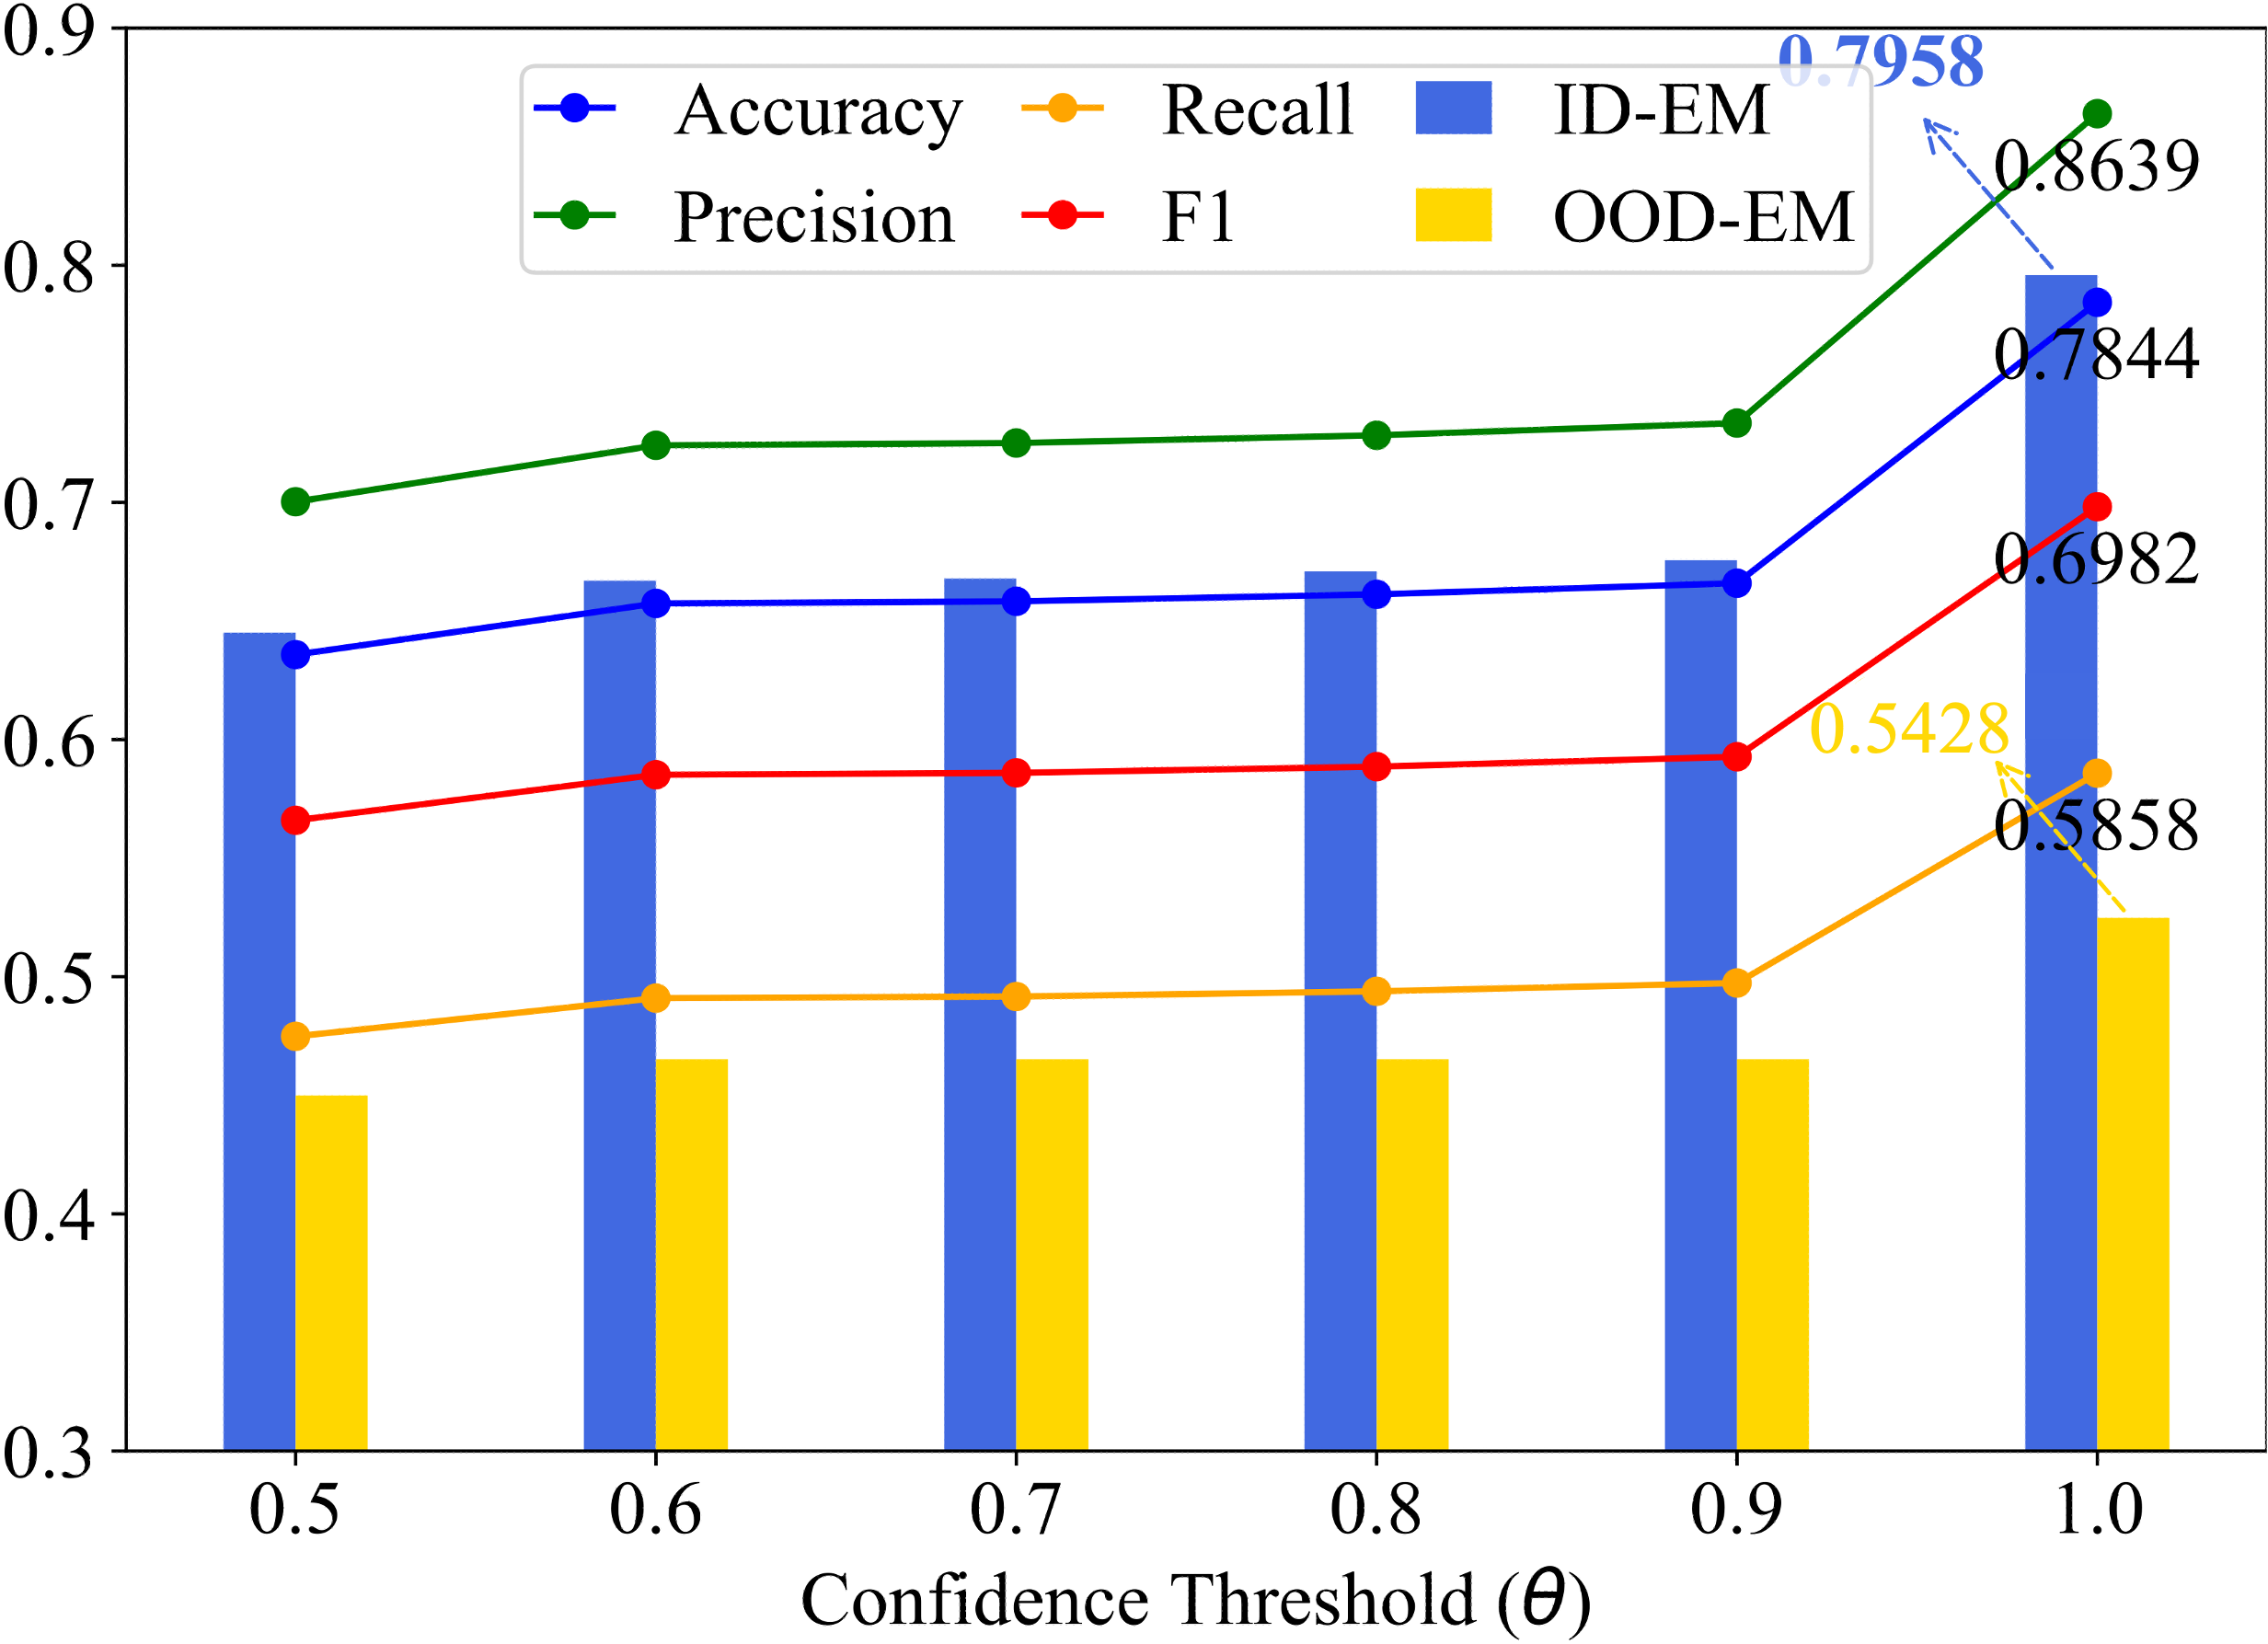
\includegraphics[width=0.465\textwidth]{fig_outlined/independent.png}
  \caption{Routing as the VLM pool evolves. Left: incremental training under
  different proportions of data from the original pool. Right: independent training
  under different cascade thresholds. The strategies respond differently to
  data imbalance and confidence.}
  \label{fig:extension}
\end{figure*}

\begin{figure*}[t]
  \centering
  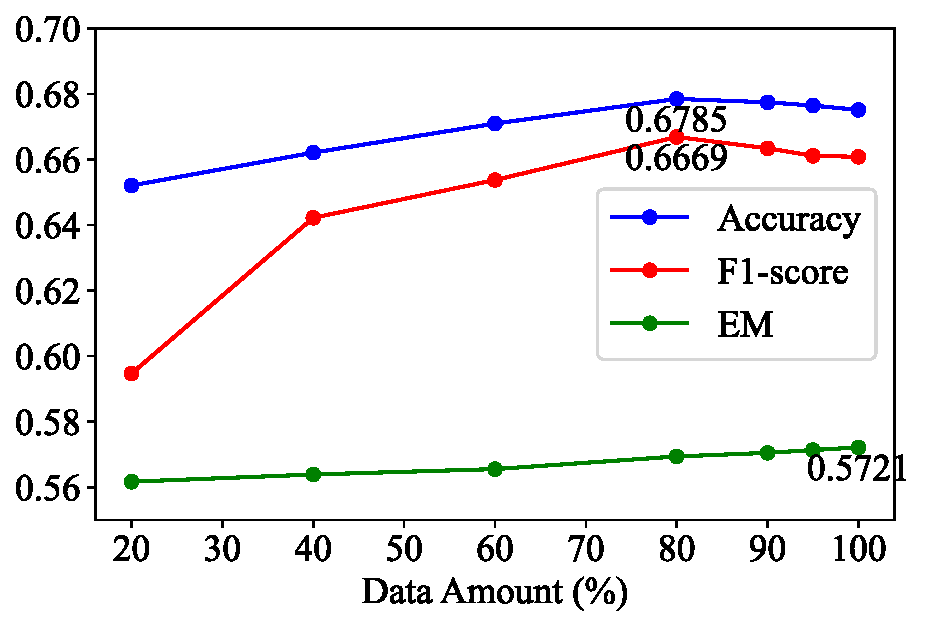
\includegraphics[width=0.32\textwidth]{fig_outlined/samples-performance.pdf}\hfill
  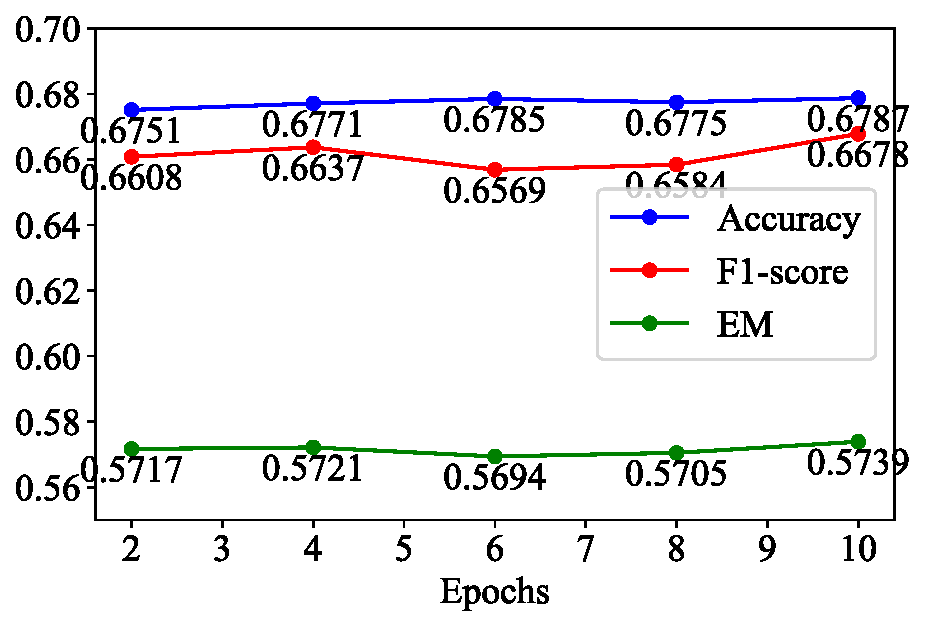
\includegraphics[width=0.32\textwidth]{fig_outlined/id_performance_epochs.pdf}\hfill
  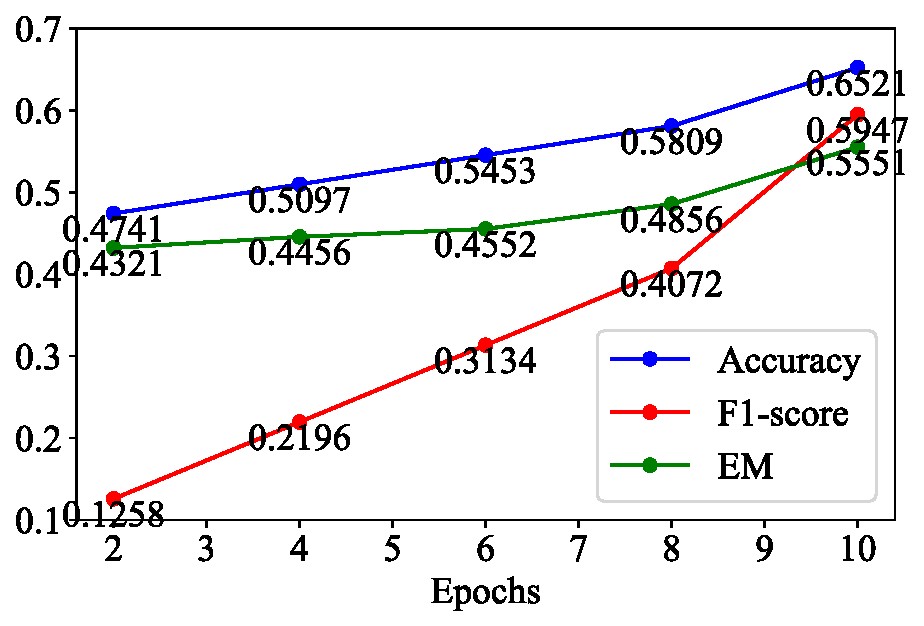
\includegraphics[width=0.32\textwidth]{fig_outlined/ood_performance_epochs.pdf}
  \caption{Robustness to training choices. Left: proportion of training data.
  Center: epochs under ID evaluation. Right: epochs under OOD evaluation.
  Additional data consistently improves answer-level EM, whereas additional
  epochs mainly benefit transfer to OOD queries.}
  \label{fig:sensitivity}
\end{figure*}

\begin{figure*}[t]
  \begin{minipage}[t]{0.48\textwidth}
    \centering
    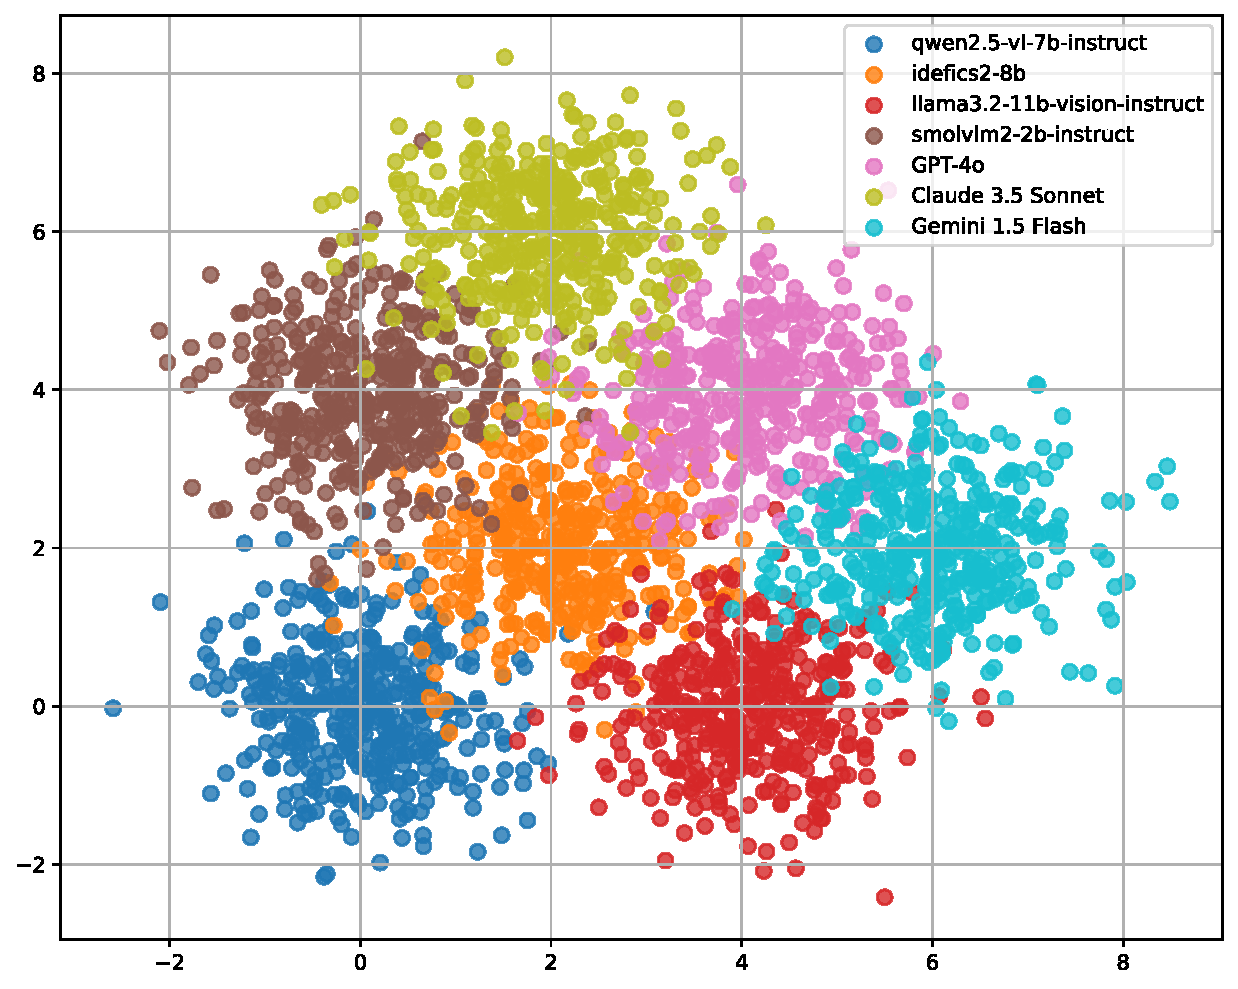
\includegraphics[width=0.86\linewidth]{fig_outlined/VLM_clusters.pdf}
    \vspace{-3mm}
    \captionof{figure}{t-SNE of fused query representations colored by selected
    VLM. Clusters encode suitability structure.}
    \label{fig:representation-vlm}
  \end{minipage}\hfill
  \begin{minipage}[t]{0.48\textwidth}
    \centering
    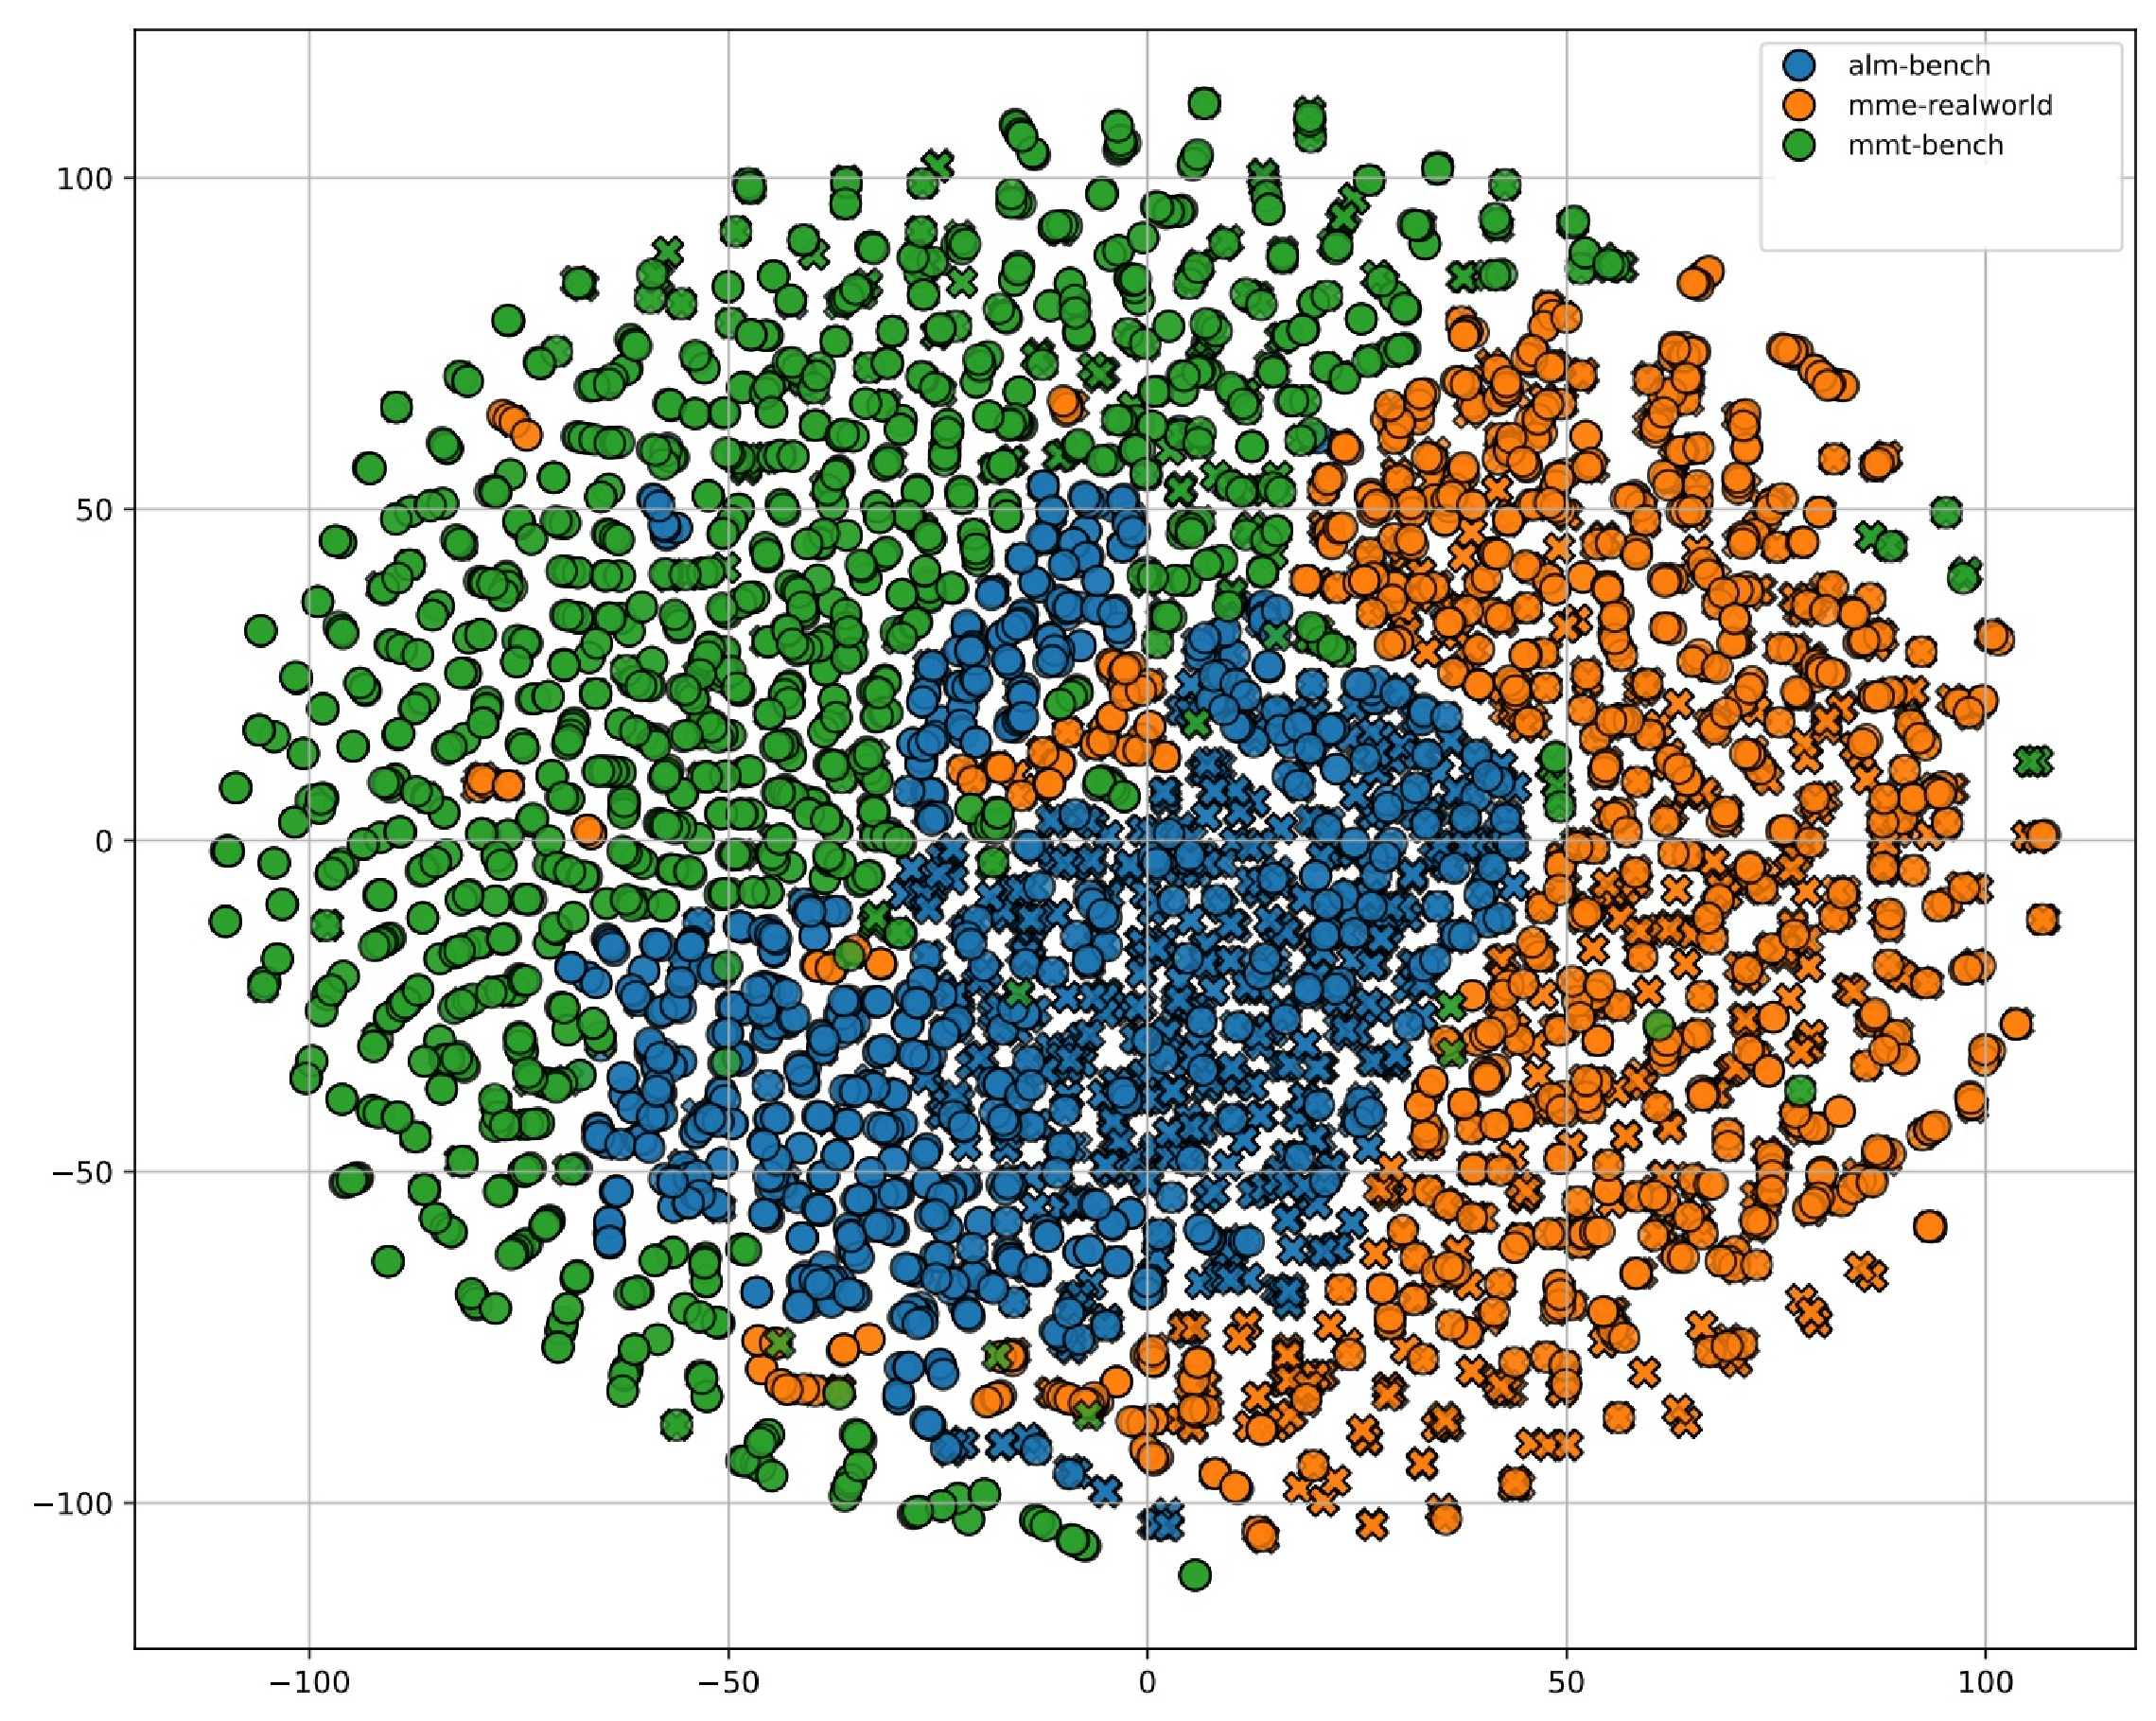
\includegraphics[width=0.86\linewidth]{fig_outlined/visual-benchmark.pdf}
    \vspace{-3mm}
    \captionof{figure}{The same t-SNE colored by source benchmark. Domain
    structure remains visible.}
    \label{fig:representation-benchmark}
  \end{minipage}
\end{figure*}

\section{Experiments}

\subsection{Evaluation Setting}

We derive ID queries from ALM-Bench \citep{ALM-bench}, MMT-Bench
\citep{MMT-Bench}, and MME-RealWorld \citep{MME-RealWorld}. OOD queries come
from VHELM \citep{VHELM}. This filtering rule is applied separately to each
candidate pool; all reported results are therefore conditional on at least one
correct candidate. The original pool
contains Qwen2.5-VL-7B \citep{qwen2.5},
Idefics2-8B \citep{idefics2}, Llama-3.2-11B-Vision \citep{llama3.2}, and
SmolVLM2-2B \citep{smolvlm2}. The evolved seven-model pool adds GPT-4o
\citep{gpt4o}, Claude 3.5 Sonnet \citep{claude}, and Gemini 1.5 Flash
\citep{gemini}.
Table~\ref{tab:data} reports query counts. Each query produces one binary outcome
per candidate in its pool.

\begin{table}[t]
\centering
\begin{tabular}{llrr}
\toprule
Split & Candidate pool & Train & Test\\
\midrule
ID  & Original: 4 VLMs & 29,626 & 3,000\\
ID  & Evolved: 7 VLMs  & 5,500  & 1,500\\
OOD & Original: 4 VLMs & --     & 7,084\\
OOD & Evolved: 7 VLMs  & --     & 9,397\\
\midrule
Total & & 35,126 & 20,981\\
\bottomrule
\end{tabular}
\vspace{-3mm}
\caption{Routing splits derived from benchmarks for the original four-model pool and
the evolved seven-model pool. The two settings use different query sets and are
evaluated separately.}
\label{tab:data}
\end{table}

The primary metric is answer-level Exact Match (EM): the fraction of queries for
which the selected candidate returns the exact answer, following HELM
\citep{HELM}. Accuracy, precision, recall, and F1 diagnose pairwise suitability
prediction. Because each retained query has at least one correct candidate, an
oracle that selects any correct candidate obtains EM 1.0 by construction. ARMS
uses CLIP-ViT-B/32 \citep{clip},
DistilBERT \citep{DistilBERT}, four experts, batch size 64, learning rate
$8\times10^{-5}$, weight decay $10^{-2}$, and AdamW \citep{AdamW}. Router
experiments use four RTX 4090 GPUs and a 16-core Xeon Gold 6430 CPU. Candidate
outputs for the open-source pool were collected on four A100 GPUs.

\paragraph{Protocol for the evolved pool.}
The term \emph{evolved pool} denotes the controlled addition of three previously
unseen VLMs to the original four-model candidate set. Table~\ref{tab:data}
also shows that the original and evolved settings use different held-out
queries. We therefore compare ARMS with baselines that always select one VLM,
evaluated on the same queries within each setting; we do not interpret the raw difference
between the four- and seven-model scores as a causal gain from pool growth.
Incremental and independent training, by contrast, are evaluated on the same
split for the evolved pool and can be compared directly. OOD labels are never used for
training or threshold selection.

\paragraph{Implementation and inference.}
The encoders for the question and candidate descriptions produce 768-dimensional
vectors, while CLIP produces 512-dimensional visual tokens. The four
cross-attention experts share the encoded query, and all candidate descriptions
are cached before selection. Open-source candidate outputs are generated with
bfloat16 weights, each processor's chat template, a maximum of 16 new tokens,
and deterministic greedy decoding. Router training applies binary
cross-entropy to every query-candidate label. At evaluation, ARMS scores all
candidates, chooses the largest score, and then reads the corresponding cached
candidate outcome. Thus every router and baseline that selects one fixed VLM within a
setting is evaluated against the same answer records.

\paragraph{Metric interpretation.}
{\hyphenpenalty=10000
Pairwise Accuracy and F1 measure whether the router recognizes every suitable
query-candidate pair, while EM measures the correctness of the single candidate
chosen by the argmax. They answer different questions. If several VLMs answer a
query correctly, misclassifying one positive pair need not reduce EM as long as
another correct candidate receives the largest score. Conversely, one highly
ranked false positive can reduce EM despite otherwise accurate pairwise
predictions. We therefore treat EM as the primary system outcome and use
classification metrics to diagnose why selection succeeds or fails. This also
motivates the oracle, which quantifies pool complementarity rather than the
performance of the learned router.\par}

\subsection{Results as the VLM Pool Evolves}

Figure~\ref{fig:main} compares ARMS with assigning every query to one fixed VLM.
For four open-source candidates, ARMS reaches 0.5739 ID and 0.4321 OOD EM after
two epochs, exceeding each individual VLM. In the separately evaluated,
evolved seven-model pool, independent training reaches 0.7958 ID and 0.5428 OOD
EM. Because the four- and seven-model settings use different test query sets,
these scores characterize performance within each setting rather than a causal
gain from adding models. ARMS's advantage over the fixed candidates within each
setting shows that it exploits complementary competence rather than producing
answers itself. The remaining gap to the oracle also shows that candidate
selection is not solved.

Independent training is consistently stronger than incremental training for the
evolved heterogeneous pool. Incremental updates reuse the original router but
expose it to substantially fewer examples for the added VLMs, so the imbalance
between original and added data limits adaptation. Independent training isolates
the added subset and avoids this interference. Its threshold cascade is stable for
$\theta\in[0.5,0.9]$, with stricter routing at $\theta=1.0$ further improving
all selection metrics.

Figure~\ref{fig:extension} explains the gap between the two strategies.
Incremental training performs best when supervision for the original and added
candidates is relatively balanced. As the original portion
grows, gradients from the added candidates become a smaller fraction of the
update and EM declines. Independent training removes this competition. $\Theta$
learns only the added subset, and the cascade delegates difficult decisions
according to $\theta$. Its broad plateau over $[0.5,0.9]$ indicates that the
gain is not tied to a narrowly tuned threshold. These observations support
independent training when a heterogeneous pool evolves with scarce data for
added VLMs, and incremental training when supervision for the original and added
VLMs is balanced.

\subsection{Ablation and Robustness}

Table~\ref{tab:ablation} isolates the principal components. Restoring the full
candidate description in place of the model name raises EM from 0.5115 to
0.5721, an absolute gain of 0.0606.
Replacing cross-attention with concatenation reduces F1 and EM, confirming that
interactions between visual and textual features cannot be captured by a fixed
merge. Freezing the text
encoder causes the largest degradation, which is consistent with both the
question and the model descriptor carrying essential textual evidence.

All ablations share the same split and argmax rule, so their differences are
directly comparable. The full description adds 0.0606 EM over an input containing
only the model name, gated cross-attention adds 0.0449 over concatenation, and training the
text encoder adds 0.2241 over freezing it. These gaps isolate the contributions
of model information, multimodal interaction, and adaptable textual features.

\begin{table}[t]
\centering
\setlength{\tabcolsep}{4pt}
\begin{tabular}{lccc}
\toprule
Variant & Accuracy & F1 & EM\\
\midrule
Freeze image               & 0.6542 & 0.6452 & 0.5351\\
Freeze text                & 0.5875 & 0.4631 & 0.3480\\
Concatenation              & 0.6577 & 0.6036 & 0.5272\\
Model name only            & 0.6254 & 0.6168 & 0.5115\\
ARMS                       & \textbf{0.6751} & \textbf{0.6634}
                           & \textbf{0.5721}\\
\bottomrule
\end{tabular}
\vspace{-3mm}
\caption{Component ablation on the four-candidate ID split. ``Model name only''
replaces the full candidate description with the model name; the parenthetical
value is the absolute EM gain from restoring the description.}
\label{tab:ablation}
\end{table}

Increasing the training fraction improves answer-level EM even after pairwise
classification metrics saturate. Additional epochs change ID EM only from
0.5717 to 0.5739 but raise OOD EM from 0.4321 to 0.5551, an absolute gain of
0.1230. This suggests that longer optimization mainly improves
transferable routing patterns.

Figure~\ref{fig:sensitivity} separates answer-level routing quality from
pairwise classification quality. Accuracy and F1 peak near 80\% of the training
data, but EM continues to improve with more data. A router can therefore improve
the final answer stream even when a global binary metric saturates. Errors on
queries with multiple correct candidates need not alter the selected answer,
whereas a small score change can switch a query from an incorrect to a correct
candidate. The epoch curves show a second distinction. ID performance saturates
quickly, but OOD EM improves by 28.47\% relative, suggesting that longer
optimization refines cross-modal patterns that transfer beyond the training
benchmarks.

\subsection{Representation Analysis}

We inspect the fused vectors $e_i$ using t-SNE only as a qualitative diagnostic,
not as evidence of causal specialization. Figures~\ref{fig:representation-vlm}
and~\ref{fig:representation-benchmark} show structure by selected VLM and source
benchmark. The coloring by selected VLM indicates that the representation
contains information about which models suit each query, while the coloring by
benchmark shows that it preserves variation across query sources. This
organization is consistent with
the ablation results. Removing candidate descriptions reduces EM, and replacing
cross-attention with concatenation weakens routing. The visualizations do not
prove expert specialization, but they check that ARMS learns more than generic
text semantics.

\section{Conclusion}

ARMS frames VLM selection as multimodal prediction guided by explicit
descriptions of each candidate's capabilities. Gated cross-attention matches
query evidence to candidate descriptions, and two training strategies add VLMs
without full joint retraining as the pool evolves. In separate evaluations of
the original and evolved pools, ARMS improves answer accuracy over every fixed
candidate on ID and OOD queries for which at least one candidate is correct.
The shared scorer is invariant to candidate order and pool size. The reported
gains apply to the pre-invocation, answerable-query setting: EM evaluates
selection when a correct candidate exists rather than abstention when all
candidates fail, and reliable routing to added VLMs still uses outcome
supervision.

% The review source uses a bibliography in which the authors' prior work is
% masked.  The camera-ready source switches this back to arms_aaai.bib.
\newpage
\bibliography{arms_aaai_anonymous}

\end{document}
